This section discusses the detailed methodology of creating motion features, particularly, ``Motion tubes'', ``HOOF'', and ``BoW'' blocks as illustrated in Fig. \ref{fi:overall}.

\subsubsection{Low level motion descriptor}
A pixel level descriptor is required to identify moving points in the video. Dense trajectories \cite{wang2011action} is a powerful
pixel-level algorithm, which captures and tracks motion across several frames. In this work
we choose dense trajectories as the low level descriptor for capturing raw motion.

\subsubsection{Clustering}

Initially we create dense trajectories for every frame in the video.
Then in order to isolate each sub area in a frame which contains significant motion we apply DBScan clustering on the calculated trajectory points.
Algorithm~\ref{alg:Clustering algorithm}  illustrates our clustering approach. Empirically, we use 8 and 10 as $\epsilon$ and MinPoints parameters respectively.



\begin{algorithm}
 \caption{DBScan Clustering algorithm.}
   \label{alg:Clustering algorithm}
    \begin{algorithmic}[1]
    \Require  $\mathcal{D}$ \Comment{Data set of sub-areas in frame}
    \Require $M$ \Comment{minimum no. of points}
    \Require $\epsilon$ \Comment{$\epsilon$  parameter}
      %\Function{dbScan}{DataSet, $\epsilon$, MinPoints}
        \State $c \leftarrow 0$ \Comment{initialize cluster no.}
        \ForEach {$P \in$ $\mathcal{D}$}
	  \If{$P$ is $visited$}
	    \State{\textbf{continue}}
	  \EndIf
            \State mark $P$ as $visited$
            \State NeighborPts = \textsc{getAllPoints}($P$, $\epsilon$)
          \If{size(NeighborPts) $< M$}
          \State{mark $P$ as noise}
          \Else
          \State{$c$ = next cluster}
          \State{\textsc{addToCluster}($P$, NeighborPts, $c$, $\epsilon$, $M$)}
          \EndIf
        \EndFor
       %\EndFunction

       \Function{addToCluster}{$P$, NeighborPts, c, $\epsilon$, MinPoints}
	\State add $P$ to cluster $c$
	\ForEach  {point $np \in$ NeighborPts}
	  \If{$P$ is not $visited$}
	    \State mark $np$ as $visited$
	    \State NeighborPts' = \textsc{getAllPoints}($np$, $\epsilon$)
	    \If {size(NeighborPts) $\geq$ MinPoints}
            \State NeighborPts' $\leftarrow$ NeighborPts joined with NeighborPts'
            \EndIf
	
	  \EndIf
	  \If{$np$ is not yet member of any cluster}
         \State add $np$ to cluster $c$
         \EndIf
	\EndFor
       \EndFunction

       \Function{getAllPoints}{$P$, $\epsilon$}
       \Return all points within $P$'s $\epsilon$-neighborhood (including $P$)
       \EndFunction
\end{algorithmic}

\end{algorithm}


Despite the presence of many regions which contain motion in a video, some are neither significant nor descriptive.
Those moving regions can be neglected without loss of performance. Therefore after clustering each trajectory point in to cluster groups non-significant cluster groups are neglected.
We do this in order to prevent the algorithm focusing on small random moving areas in a video as well as to limit creation of motion tubes to areas which are significant and descriptive.
Therefore all the clusters which are not at least 50\% of the largest cluster of the frame are discarded.

After identifying the initial candidate clusters for creating action boxes further processing is done to each cluster to ensure that they contain only the important moving areas according to Algorithm~\ref{alg:boundary removal}. For each point the Chebychev distance from the centroid of the cluster is calculated as in
Eq. \ref{eq:chebichev}. We discard the furthest 20\% of the points from the cluster. The reason behind the choice of Chebychev distance over Euclidean distance is due to the possibility of obtaining symmetric square shaped cluster groups as opposed to circular ones. This makes it easier to track moving areas and create motion tubes.

\begin{equation}\label{eq:chebichev}
 D_{Chebychev} = \max(|X_{2} - X_{1}|,|Y_{2}-Y_{1}|)
\end{equation}

\begin{algorithm*}
   \caption{Boundary noise removal algorithm of clusters.}
   \label{alg:boundary removal}
    \begin{algorithmic}[1]
     \Function{formatCluster}{inCluster, maxChebichevDistance}
	\State {$M_{d}$ = maxChebichevDistance}
	\State {totalPoints = \textsc{getTotalPoints}(inCluster, $M_{d}$)}
	\State {currentPoints $=$ totalPoints}
	\While{$true$}
	  \If{\textsc{count}(currentPoints) $<$ \textsc{count}(totalPoints) $\times80/100$}
	    \State {$return$ all the points bellong to currentPoints}
	  \EndIf
	  \State {$M_{d}= M_{d} - 1$}
	  \State {currentPoints $=$ \textsc{getTotalPoints}(inCluster, $M_{d}$)}
	
	\EndWhile
     \EndFunction


\end{algorithmic}
\end{algorithm*}

After identifying square-shaped interest regions (action boxes), we represent each of them with a vector, $b = (x,y,r,f)$, where $x$ and $y$ are the coordinates
of the top left corner of the box, $r$ is the height or width of the box, and $f$ is the frame number.


\subsubsection{Motion Tubes}
Since our work models the time evolution of sub activities within a video, we divide each input video $V_{i}$ into temporal segments, $f(V_{i}) = [v_{i,1},
v_{i,2}, \dots, v_{i,n}]$,
and create features for each individual segment separately. Therefore, after creating the action boxes for each video segment,
the action boxes within a segment $v_{i,t}$ can be represented as,

\begin{equation}
\label{eqn:action box}
\begin{split}
\MoveEqLeft
 g(v_{i,t}) = \big\{[b_{t,1,1},b_{t,1,2},\dots,b_{t,1,q}],\\
 & [b_{t,2,1},b_{t,2,2},\dots,b_{t,2,p}],\dots,[b_{t,n,1},b_{t,n,2},\dots,b_{t,n,k}]\big\}
\end{split}
\end{equation}

where $b_{t,j,k}$ is the $k^{th}$ action box in $j^{th}$ frame of the $t^{th}$ video segment. Note that the number of
action boxes differ from frame to frame.

Therefore before linking the action boxes to create motion tubes further pre processing is needed to ensure the same number of action
boxes exist in every frame within a video segment. Otherwise, different motion tubes could become joined halfway through the video and the
effort to capture dynamics of each moving object separately is disturbed.

First we calculate the mean number of action boxes per frame in each segment. Then we obtain the rounded down value, $N$, of that number.
Afterwards, we iterate through each frame starting from frame number $1$ until we come to a frame $W$ which has $N$ number of action boxes.

Then from frame $W$ we propagate forward and backward along the frames, either to eliminate or add action boxes. The procedure is explained below.

If the action box count in a particular frame is larger than the previous frame the smallest excess number of action boxes are removed.
In the case where the action box count is lower than the previous frame, linear regression (Eq. \ref{eqn:linear regression}) is used for each $x,y$ and $r$ value of vector $b = (x,y,r,f)$
up to that frame, in order to create artificial action boxes until the number of action boxes matches $N$.

\begin{equation}
\label{eqn:linear regression}
\begin{bmatrix}
    Y_{1}     \\
    Y_{2}     \\
    \hdotsfor{1} \\
    Y_{n}
\end{bmatrix}
=
\begin{bmatrix}
    1 & X_{1}     \\
    1 & X_{2}     \\
    \hdotsfor{2} \\
    1 & X_{n}
\end{bmatrix}
*
\begin{bmatrix}
    \beta_{0}     \\
    \beta_{1}
\end{bmatrix}
+
\begin{bmatrix}
    \epsilon_{1}     \\
    \epsilon_{2}    \\
    \hdotsfor{1} \\
    \epsilon_{n}
\end{bmatrix}
\end{equation}

where $Y$ and $X$ would be either $x,y$ or $r$. Then least squares method is used to minimize the error, $\sum{\epsilon^2}$, and find the
values for $\beta_{1}$ and $\beta_{0}$. Afterwards, using these values missing action boxes are predicted.
Note that $n$ increases as the observed action boxes
increase; hence the prediction becomes more accurate. Note how this processing results in Eq. \ref{eqn:action box}
being transformed in to Eq. \ref{eqn:action box transformed},
thus verifying that the number of action boxes per frame is equal for all frames within a video segment.

\begin{equation}
\label{eqn:action box transformed}
\begin{split}
\MoveEqLeft
 h(g(v_{i,t})) = \big\{[b_{t,1,1},b_{i,1,2},\dots,b_{t,1,k}],\\
 & [b_{t,2,1},b_{t,2,2},\dots,b_{t,2,k}],\dots,[b_{t,n,1},b_{t,n,2},\dots,b_{t,n,k}]\big\}
\end{split}
\end{equation}


The following procedure is used to link the action boxes in consecutive frames.

Assume $b_{t,k,1}$,$b_{t,k,2}$,\dots,$b_{t,k,n}$ and $b_{t,k+1,1}$,$b_{t,k+1,2}$,\dots,$b_{t,k+1,n}$  are action boxes in two
consecutive frames at time $k$ and $k+1$. Then the following distance matrix is calculated.



\begin{equation}
D=\begin{bmatrix}
    D_{11}       & D_{12} & D_{13} & \dots & D_{1k} \\
    D_{21}       & D_{22} & D_{23} & \dots & D_{2k} \\
    \vdots       & \vdots & \vdots & \vdots & \vdots \\
    D_{k1}       & D_{k2} & D_{k3} & \dots & D_{kk}
\end{bmatrix}
\end{equation}


where $D_{i,j}$ is the Euclidean distance between the centroids of $i^{th}$ action box in $k^{th}$ frame and $j^{th}$ action box in $(k+1)^{st}$ frame.
Then $u^{th}$ action box at $k+1$, and $1^{st}$ action box at $k$ is linked, where $u$ is calculated using,


\begin{equation}
u=\underset{j\in J}{\mathrm{argmin}_j}\{D_{1,j}\}, J=\{1,2,\dots,l\}
\label{link eq}
\end{equation}

Then the $1^{st}$ row and the $u^{th}$ column are removed from the distance matrix, and we apply the same process repeatedly using Eq. \ref{link eq}
to link each of the action boxes at $k$ with $k+1$.

By this removal process, we avoid combining of motion tubes half-way through
the video segment and keep them isolated from each other, which is vital for capturing the dynamics separately for each moving object.




Finally, we create matrix $M_{i}$ which encodes all the information of motion tubes, in a particular video segment.
\begin{equation}
M=\begin{bmatrix}
    1       & 1 & x_{1,1} & y_{1,1} & r_{1,1} \\
    1       & 2 & x_{1,2} & y_{1,2} & r_{1,2} \\
    \vdots       & \vdots & \vdots & \vdots & \vdots \\
    1       & n & x_{1,n} & y_{1,n} & r_{1,n} \\
    2       & 1 & x_{2,1} & y_{2,1} & r_{2,1} \\
    2       & 2 & x_{2,2} & y_{2,2} & r_{2,2} \\
    \vdots       & \vdots & \vdots & \vdots & \vdots \\
    2       & n & x_{2,n} & y_{2,n} & r_{2,n} \\
    \vdots       & \vdots & \vdots & \vdots & \vdots \\
    z       & 1 & x_{z,1} & y_{z,1} & r_{z,1} \\
    z       & 2 & x_{z,2} & y_{z,2} & r_{z,2} \\
    \vdots       & \vdots & \vdots & \vdots & \vdots \\
    z       & n & x_{z,n} & y_{z,n} & r_{z,n} \\

\end{bmatrix}
\end{equation}

where the columns represent the frame number, action box number, $x$ coordinate of the top left corner,
$y$ coordinate of the top left corner, and the width/height of the action box, respectively.

\subsubsection{Histogram Oriented Optic Flows (HOOF)}
Since each action box in a particular motion tube may differ in size, we take $R = \max(r_{i})$, for $\forall{i}$,
where $r_{i}$ is the $i^{th}$ action box of the motion tube. Then we redraw the action boxes around their centroids having width or length as $R$.
After identifying the $k$ number of motion tubes ($k$ is a variable) for each video segment $v_{i,n}$, we calculate the optic flows along each motion tube
using Lucas \textit{et. al} \cite{lucas1981iterative}.
After that we create HOOF\cite{chaudhry2009histograms} for every
    action box within a motion tube. Each optic flow vector within a spatio-temporal action box within a motion tube is binned according
    to its primary angle from the horizontal axis and weighted according to its magnitude.  Therefore, all optical flow vectors, $z=[x,y]^T$ with direction,
$\theta = \tan^{-1}(\frac{x}{y})$ in the range,

\begin{equation}
- \frac{\pi}{2} + \pi\frac{b-1}{B} \leq \theta < -\frac{\pi}{2} + \pi\frac{b}{B}
\end{equation}

will contribute a weight of $\sqrt{x^2 + y^2}$ to the sum in bin $b$, $1 \leq b \leq B$ out of a total of
$B$ bins. Finally, the histogram is normalized. We choose 100 number of bins. Example HOOF creation for 6 bins is illustrated in Fig. \ref{fi:hoof}.

\subsubsection{Bag of HOOFs}
We use a bag of features method to create a motion descriptor for each video segment. First, we create a code book for HOOF vectors.
100,000 vectors are randomly selected from all the HOOF vectors of all the video segments in all video classes.
Then these 100,000 vectors are clustered using $k$-means clustering and 1000 cluster heads
are identified. We choose the number of cluster heads as 1000, because the dimensions of final motion descriptors are needed to be the same as
the static descriptors, which is explained in section V. Then for each video segment $v_{i,n}$, a histogram is calculated as follows.


we calculate,
\begin{equation}
p = \underset{j\in J}{\mathrm{argmin}_{j}}(T_{j}-h_{n,k}), J=\{1,2,\dots,1000\}
\end{equation}

for each $k$ in $\{1,2,\dots, l\}$, where $h_{n,k}$ is the $k^{th}$ HOOF vector of the $n^{th}$ video segment, and $T_{j}$ is the $j^{th}$ cluster head. Then we increment the histogram values as,

\begin{equation}
H_{n}(p) = H_{n}(p)+1
\end{equation}
where $H_{n}(p)$ is the $p^{th}$ value, $1<p<1000$, of histogram of the $n^{th}$ video segment $v_{i,n}$. After calculating the histogram vector $H_{n}$ for every video segment $v_{i,n}$
this $H = [H_{1},H_{2}, \dots, H_{n}]$ is the vector time series, which encodes the time evolution of motion information in the video.

\begin{figure}
  \centering
  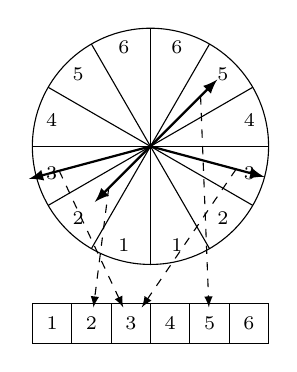
\begin{tikzpicture}[x=1cm, y=1cm, every node/.append style={text=black, font=\scriptsize}]
\def\r{1.5}
	\draw (0,0) coordinate (o) circle (\r);
	\foreach \theta in {-90, -60, ..., 240}
	{
		\draw (o) -- (\theta:\r);
	}
	\foreach \theta/\l in {-60/1, -30/2, 0/3, 30/4, 60/5, 90/6}
	{
		\node at  (\theta - 15:1.3) {$\l$};
	}	
	\foreach \theta/\l in {-90/1, -120/2, -150/3, -180/4, -210/5, -240/6}
	{
		\node at  (\theta - 15:1.3) {$\l$};
	}		
	
	\foreach \theta/\r/\t in {-15/1.5/1, 45/1.2/2, -135/1/3, -165/1.6/4}
	{
		\draw[-latex, thick] (o) -- (\theta:\r ) coordinate [near end] (t\t);
	}
	
	\foreach \i/\l in {-1.25/1, -0.75/2, -0.25/3, 0.25/4, 0.75/5, 1.25/6 }
	{
		\draw (\i-0.25, -2) rectangle ++(0.5, -0.5);
		\node (a\l) at (\i, -2.25) {$\l$} ;
	}
	
	\draw[-latex, dashed] (t1) -- (a3);
	\draw[-latex, dashed]  (t2) -- (a5);
	\draw[-latex, dashed]  (t3) -- (a2);
	\draw[-latex, dashed]  (t4) -- (a3);
	
	
\end{tikzpicture} 
  \caption{Example HOOF generation with 6 bins}\label{fi:hoof}
\end{figure}
